\subsubsection{Pixel Formats}
\label{subsubsec:pixel_format}
\todo[inline]{Citations, Include general naming scheme (RGGB, GRBG, GBRG and BGGR) right before the Baumer one?, Document that only 8bits are used?}

The Baumer industrial camera VCXU-13C uses the digital image sensor PYTHON1300 from ON Semiconductor and allows for the use of monochrome, raw and color pixel formats (see chapter \ref{sec:camera}).
The digital image sensor itself has 1280 $\times$ \SI{1024}{px} that aquire brightness with a bit depth of \SI{10}{bit}.
In order to capture color images, a color filter is applied to each individual pixel.
These red, green and blue (RGB or BGR) color filters only transmit light with a particular wavelength.
Due to the fact that the luminance perception of the human eye is most sensitive to green light, twice as many green filters are used as red and blue filters.
The color filters are arranged in a Bayer color matrix $B$, as shown in figure \ref{subfig:bayerrg}.
% https://www.cambridgeincolour.com/tutorials/camera-sensors.htm
% (https://en.ids-imaging.com/tl_files/downloads/techtip/TechTip_18MP-color-sensor-as-mono_EN.pdf)

\begin{figure}[H]
  \centering
  \begin{subfigure}[b]{0.3\textwidth}
    \centering
    \includegraphics[scale=1]{bayerrg}
    \caption{Baumer \texttt{BayerRG}}
    \label{subfig:bayerrg}
  \end{subfigure}
  \begin{subfigure}[b]{0.3\textwidth}
    \centering
    \includegraphics[scale=1]{bayergr}
    \caption{Baumer \texttt{BayerGR}}
    \label{subfig:bayergr}
  \end{subfigure}
  \begin{subfigure}[b]{0.3\textwidth}
    \centering
    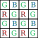
\includegraphics[scale=1]{bayergb}
    \caption{Baumer \texttt{BayerGB}}
    \label{subfig:bayergb}
  \end{subfigure}
  \caption{Bayer color matrices $B$}
  \label{fig:bayer}
\end{figure}

There are several modifications of the Bayer pattern that can be achieved by simply shifiting the pixels around.
The pattern in figure \ref{subfig:bayergr} is achieved by shifting the initial pattern one pixel to the left, whereas the pattern in figure \ref{subfig:bayergb} is achieved by shifting the pattern one pixel up.

Furthermore, there exist different naming conventions for the different Bayer patterns.
Baumer labels the Bayer patterns after the color of the elements $B_{11}$ and $B_{12}$, resulting in the name \texttt{BayerRG} for figure \ref{subfig:bayerrg}.
However, the Open Computer Vision Library (OpenCV) labels it after the elements $B_{22}$ and $B_{23}$, resulting in the name \texttt{BayerBG} for the same figure \ref{subfig:bayerrg}.
% https://www.baumer.com/ch/en/service-support/know-how/technical-information-industrial-cameras/baumer-gapi-and-opencv/a/baumer-gapi-and-opencv

In order to create an RGB color image from the raw Bayer pattern image, a demosaicing (also ``debayering'') algorithm is necessary.
The Baumer industrial camera VCXU-13C is able to transform the raw sensor data into the respective RGB or BGR values in real time.
Another possibility is to do the required color space transformation with the OpenCV function \texttt{cv::cvtColor}.
The required color space conversion code is \texttt{cv::COLOR\_BayerBG2BGR}.
This will convert the raw Bayer pattern image into a BGR image (OpenCV uses the BGR instead of the standard RGB color space).
% https://docs.opencv.org/4.1.1/d8/d01/group__imgproc__color__conversions.html#ga397ae87e1288a81d2363b61574eb8cab
